\documentclass{article}
\usepackage{pgfplots}
\usepackage{pgfplotstable}
\usepackage{graphicx}
\usepackage{multicol}
\usepackage{enumerate}
\pgfplotsset{compat=1.16}
\usetikzlibrary{matrix,chains,trees,scopes,decorations}
\usetikzlibrary{arrows.meta,automata,positioning,shadows,3d}
\usetikzlibrary {decorations.pathmorphing}
\usetikzlibrary {backgrounds,mindmap,shadows}
\usetikzlibrary {patterns, quotes}
\usetikzlibrary {graphs,fadings}
\usetikzlibrary {arrows,shapes.geometric}
\usepgflibrary {shadings}




\title{TikZ Overview}
\author{Eureka}
\date{\today}
\begin{document}
\maketitle




\section{Shading and Highligh}

\begin{tikzpicture}
    \tikz\shade (0,0) rectangle (2,1) (3,0.5) circle (.5cm);
\end{tikzpicture}
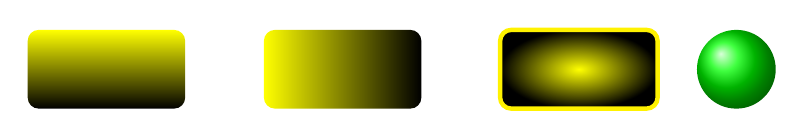
\begin{tikzpicture}[rounded corners,ultra thick]
    \shade[top color=yellow,bottom color=black] (0,0) rectangle +(2,1);
    \shade[left color=yellow,right color=black] (3,0) rectangle +(2,1);
    \shadedraw[inner color=yellow,outer color=black,draw=yellow] (6,0) rectangle +(2,1);
    \shade[ball color=green] (9,.5) circle (.5cm);
\end{tikzpicture}

\section{Path Decoration}




\section{Path}
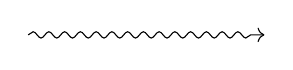
\begin{tikzpicture}
    \draw [
        ->,decorate,
        decoration={snake,amplitude=.4mm,segment length=2mm,post length=1mm}
    ]
    (0,0) -- (3,0);
\end{tikzpicture}




\section{A Special Example}
\begin{figure}[!htb]
    \centering
    \rotatebox{90}{
        \includegraphics[scale=.35]{./Cover/cover.pdf}
    }
    \caption{Cover}
    \label{Cover}
\end{figure}


\section{Fill Style}
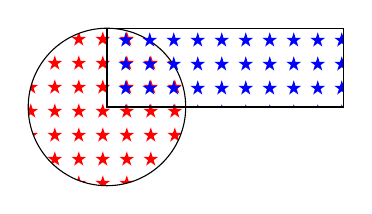
\begin{tikzpicture}
    \draw[pattern color=red,pattern=fivepointed stars] (0,0) circle (1cm);
    \draw[pattern color=blue,pattern=fivepointed stars] (0,0) rectangle (3,1);
\end{tikzpicture}
\hspace*{2.5em}
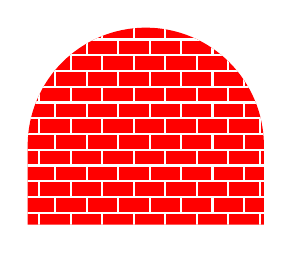
\begin{tikzpicture}
    \def\mypath{(0,0) -- +(0,1) arc (180:0:1.5cm) -- +(0,-1)}
    \fill [red] \mypath;
    \pattern[pattern color=white,pattern=bricks] \mypath;
\end{tikzpicture}
\hspace*{2.5em}

\begin{tikzpicture}
    \node [circular drop shadow={shadow scale=1.05},minimum size=3.13cm,
    decorate, decoration=zigzag,
    fill=blue!20,draw,thick,circle] {Hello!};
\end{tikzpicture}


\section{Arrows and Arcs}
\tikz{
    \draw [-{Stealth[length=8mm,width=3mm]}] (0,0) -- (2,0);
    \draw [|<->|] (1.3,.4) -- node[above=1mm] {8mm} (2,.4);
    \draw [|<->|] (2,.2) --  node[right=1mm] {3mm} (2,-.2)
} 
\hspace*{5em}
\tikz{
    \draw [-{Classical TikZ Rightarrow[length=5mm]}] (0,0) -- (2,0);
    \draw [|<->|] (1.5,.6) -- node[above=1mm] {5mm} (2,.6);
}
\hspace*{5em}
\tikz{
    \draw [-{Latex[length=6mm, width=2mm]}] (0,0) -- (2,0);
    \draw [|<->|] (1.5,.4) -- node[above=1mm] {5mm} (2,.4);
    \draw [>|-|<] (2,.2) --  node[right=1mm] {2mm} (2,-.2)
}

\vspace*{3em}
\newcommand{\y}{-7}
\tikz [ultra thick] {
    \draw [arrows = {-Hooks[]}] (0,\y) -- (1,\y);
    \draw [arrows = {-Hooks[arc=90]}] (5,\y) -- (6,\y);
    \draw [arrows = {-Hooks[arc=270]}] (9,\y) -- (10,\y);
}


\vspace*{3em}
\leavevmode\raise.5em\hbox{The Following Anote can use as BookTabs}
\tikz \draw [line width=4ex,-{Triangle Cap []}](0,0) -- (1,0);
\hspace*{4em}
\tikz \draw [color=orange,line width=4ex, -{Triangle Cap[reversed]}](0,0) -- (1,0);

Words over arrow
\tikz \draw(0,0) edge ["left", ->] (2,0);



\section{WaterProof}
\begin{tikzpicture}[remember picture,overlay]
    \draw [line width=1mm,opacity=.25]
        (current page.center) circle (3cm);
    \node [rotate=60,scale=10,text opacity=0.2]
        at (current page.center) {WaterProof};
\end{tikzpicture}

\noindent\rule{.9\linewidth}{2pt}
\begin{verbatim}
    \begin{tikzpicture}[remember picture,overlay]
        \draw [line width=1mm,opacity=.25]
            (current page.center) circle (3cm);
        \node [rotate=60,scale=10,text opacity=0.2]
            at (current page.center) {WaterProof};
    \end{tikzpicture}
\end{verbatim}


\clearpage
\section{Ball Drawing}
% \tikz\draw[shading=ball] (0,0) circle(3pt);

% 命令封装
\newcommand{\ball}{\leavevmode\raise.1em\hbox{\tikz\shade[ball color=red] (0,0) circle (2pt);}}
Use Enumerate package To chaneg The Deafault item Style

\begin{multicols}{2}
\begin{enumerate}[\ball]
    \item The First
    \item The Second
\end{enumerate}

\newcommand{\bt}{\leavevmode\raise.1em\hbox{\tikz\draw[line width=3pt,-{Triangle Cap []},orange] (0,0)--(5pt,0);}}
\begin{enumerate}[\bt]
    \item First
    \item Second
\end{enumerate}
\end{multicols}


\section{Graphs}

\tikz \graph [grow right sep] {
    a / $a=x$ --
    b / {$b=\displaystyle \int_0^1 x dx$} --
    c [draw, circle, inner sep=7mm]
};
\hspace*{6em}
\newcount\mycount
\def\lightendeepernodes{
    \pgfmathsetcount{\mycount}{
        100-20*\pgfkeysvalueof{/tikz/graphs/placement/width}
    }
    \edef\mydepth{\the\mycount}
    \tikzset{nodes={fill=red!\mydepth,circle,text=white}}
}
\tikz\graph[placement/compute position/.append code=\lightendeepernodes]
{
    a -> {
        b -> c -> d,
            e -> {
            f,
            g
        },
        h
    }
};

\section{Fading}
\begin{tikzfadingfrompicture}[name=tikz]
    \node [text=transparent!20]
    {\fontencoding{T1}\fontfamily{ptm}\fontsize{45}{45}\bfseries\selectfont
    Ti\emph{k}Z};
\end{tikzfadingfrompicture}
% Now we use the fading in another picture:
\begin{tikzpicture}
    \fill [black!20] (-2,-1) rectangle (2,1);
    \pattern [pattern=checkerboard,pattern color=black!30]
        (-2,-1) rectangle (2,1);
    \shade[path fading=tikz,fit fading=false,
        left color=blue,right color=black]
        (-2,-1) rectangle (2,1);
\end{tikzpicture}
\hspace*{3em}
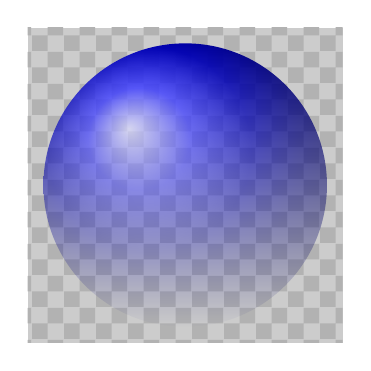
\begin{tikzpicture}
    % Checker board
    \fill [black!20] (0,0) rectangle (4,4);
    \path [pattern=checkerboard,pattern color=black!30] (0,0) rectangle (4,4);
    \shade [ball color=blue,path fading=south] (2,2) circle (1.8);
\end{tikzpicture}
\hspace*{3em}
\tikzfading[
    name=fade inside,
    inner color=transparent!80,
    outer color=transparent!30
]
\begin{tikzpicture}
    % Checker board
    \fill [black!20] (0,0) rectangle (4,4);
    \path [pattern=checkerboard,pattern color=black!30] (0,0) rectangle (4,4);
    \shade [ball color=red] (3,3) circle (0.8);
    \shade [ball color=white,path fading=fade inside] (2,2) circle (1.8);
\end{tikzpicture}


\section{Process}
\begin{figure}[!htb]
    \centering
    \rotatebox{90}{
        \includegraphics[scale=.7]{./pics/process.pdf}
    }
    \caption{Process}
    \label{Process}
\end{figure}


\section{Animation}
\qquad Now ,TikZ can Create Animations, But The output Format only Support
{\bf .svg}. Then you should add {\ttfamily [dvisvgm]} in the document
sort like:

{\textbackslash \ttfamily documentclass[dvisvgm]{article}} .

Of curse, you need import tikzlibrary {\ttfamily animations}.To Compile it,
this is the step:
\begin{itemize}
    \item latex main.tex
    \item dvisvgm main.dvi
\end{itemize} 


% \clearpage
\section{Phylogenetic Tree}
To Use This library,you need to Compile The source file using {\ttfamily Lua\LaTeX}

\begin{figure}[!htb]
    \centering
    \includegraphics[scale=.7]{./pics/Phylogenetic.pdf}
    \caption{Phylogenetic Tree}
    \label{Phylogenetic Tree}
\end{figure}



\section{Library}
\begin{figure}[!htb]
    \centering
    \includegraphics[scale=.8]{./pics/CSTree.pdf}
    \caption{CSTree}
    \label{CSTree}
\end{figure}



\section{ color wheel}
\tikz \shade[shading=color wheel white center] (0,0) circle (1.5);
\hspace*{4em}
\tikz \shade[shading=color wheel] [even odd rule]
(0,0) circle (1.5) (0,0) circle (1);



\section{TikZ Ball}
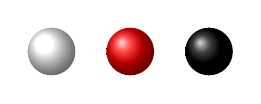
\begin{tikzpicture}
    \shade[ball color=white] (0,0) circle (2ex);
    \shade[ball color=red] (1,0) circle (2ex);
    \shade[ball color=black] (2,0) circle (2ex);
\end{tikzpicture}




\section{Shadows}
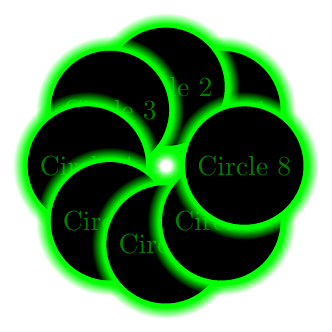
\begin{tikzpicture}
    \foreach \i in {1,...,8}
    \node[circle,circular glow={fill=green},fill=black,text=green!50!black]
    at (\i*45:1) {Circle \i};
\end{tikzpicture}
\hspace*{6em}
% \hfill
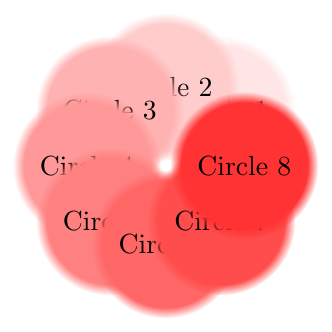
\begin{tikzpicture}
    \foreach \i in {1,...,8}
    \node[circle,circular glow={fill=red!\i0}]
    at (\i*45:1) {Circle \i};
\end{tikzpicture}


\section{Lindenmayer Pics}
\begin{figure}[!htb]
    \centering
    \includegraphics[scale=1]{./pics/Lindenmayer.pdf}
    \caption{Lindenmayer Pic}
    \label{Lindenmayer Pic}
\end{figure}





















\end{document}